% 第12章第2节：由变量消元构建动态规划（消元次序与填充图、消元簇与中间作用域、消元森林的构造、从消元簇得到树分解）。

\section{由变量消元构建动态规划}
\label{sec:graph-variable-elimination}

第~\ref{sec:graph-dp-cycle-interface}小节的消元操作每一步都产生一个新函数，它的作用域由当前所有含该变量的函数共同决定。本节说明，这些作用域可以只在原始图上模拟消元就预先算出，不需要任何函数值。按一个次序模拟一遍，就得到每一步同时处理的变量组和新函数交给哪一步使用，把它们连起来就是一个树分解。

\subsection{消元次序与填充图}
\label{sec:graph-dp-fill-in}

变量消元需要事先给定一个\term{消元次序}（elimination order）$\pi$，即全部要消去的变量的一个排列。消去一个变量时，新函数$\psi_i$的作用域$S_i$由所有含$i$的函数共同决定。在原始图上看，$S_i$恰好是$i$在当前原始图中的邻居集合，因为两个变量相邻当且仅当它们同在某个当前函数的作用域中。新函数读取这些邻居的联合取值，所以消元后的原始图中，这些邻居两两相邻。

\paragraph{一次消元的图操作}
在三元作用域例子中先消去$x_2$，就能看到这一点。$\phi_A$与$\phi_B$都含$2$，$S_2=\{1,3\}\cup\{3,4\}=\{1,3,4\}$，新函数
\[
\psi_2(x_1,x_3,x_4)=\min_{x_2}\bigl[\phi_A(x_1,x_2,x_3)+\phi_B(x_2,x_3,x_4)\bigr]
\]
同时读取$x_1,x_3,x_4$。按$(x_1,x_3,x_4)$的字典序，它的八个值为
\[
\psi_2=(3,\,2,\,0,\,+\infty,\,2,\,1,\,2,\,4),
\]
例如$(x_1,x_3,x_4)=(0,0,0)$处的两个候选为
\[
\phi_A(000)+\phi_B(000)=3,\qquad \phi_A(010)+\phi_B(100)=+\infty.
\]

原始图中原来没有边$\{1,4\}$，消元后必须补上，如图~\ref{fig:graph-dp-elimination-step}所示。这样为记录新函数的联合依赖而补入的边称为\term{填充边}（fill-in edge）。

填充边不表示原问题增加了约束，而是把原来经过$x_2$的间接联系直接记下来。看$x_3=1$的情形：$x_1=0$时，$\phi_A(0,1,1)=+\infty$迫使$x_2=0$，而$\phi_B(0,1,1)=+\infty$又禁止$x_4=1$；$x_1=1$时$x_2$可以取$1$，$x_4=1$仍然可行。原问题中$x_1$通过$x_2$牵制$x_4$。

消去$x_2$以后，这种牵制只能由$\psi_2$自己记录：上面的值中$\psi_2(0,1,1)=+\infty$，而$\psi_2(0,1,0)=0$、$\psi_2(1,1,1)=4$都有限。

若$\psi_2$能拆成一个$(x_1,x_3)$的函数与一个$(x_3,x_4)$的函数之和，固定$x_3=1$后就有
\[
\psi_2(x_1,1,x_4)=g(x_1)+h(x_4).
\]
由$g(0)+h(1)=+\infty$知$g(0)$或$h(1)$为$+\infty$，与$g(0)+h(0)$、$g(1)+h(1)$都有限矛盾。所以这张表必须同时以$x_1$和$x_4$为索引，填充边$\{1,4\}$反映的正是这一点。四环算例中消去$x_1$补入的边$\{2,4\}$也是如此（第~\ref{sec:graph-dp-four-cycle}小节）。

\begin{figure}[!htb]
  \centering
  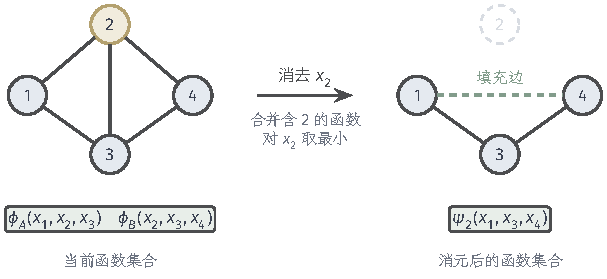
\includegraphics[width=102.687mm]{figures/01-basic-mathematics/04-graphs/tikz/c5-elimination-step/figure.pdf}
  \caption{消去$x_2$时的函数更新与图更新。左：消元前，黄色的$x_2$同时属于$\phi_A$与$\phi_B$的作用域，它的邻居是$1,3,4$。右：消元后，两个函数被新函数$\psi_2(x_1,x_3,x_4)$取代，$x_2$及其关联边被删除，邻居$1,3,4$两两相邻，其中绿色虚线$\{1,4\}$是填充边。}
  \label{fig:graph-dp-elimination-step}
\end{figure}

一般地，消元在原始图上对应一个纯粹的结构操作：把$i$的当前邻居两两连边，然后删去$i$及其关联边。不含$i$的函数提供的边保持不变；含$i$的函数在剩余变量之间提供的边都落在$S_i$内，已被补成的团覆盖；新函数$\psi_i$提供的边恰是$S_i$内的全部点对。因此，消元后函数集合的原始图恰好是对原始图执行这一操作的结果。对消元步数归纳，每一步的当前图都是当前函数集合的原始图，于是只看这个图操作，就能在不计算任何数值的情况下预先知道每一步的$S_i$。

\paragraph{填充图}
按次序$\pi$执行全部消元步骤，把途中补入的所有填充边加入原始图，得到的图称为$\pi$的\term{填充图}（filled graph），记为$\mathcal G^+_\pi$。它记录了这次消元中出现过的全部耦合：原始边来自局部函数，填充边来自中间函数。四环算例按次序$(1,2,3,4)$消元时只补入$\{2,4\}$，填充图是环加上弦$\{2,4\}$。第~\ref{sec:graph-dp-chordal}小节会说明填充图总是弦图。

\paragraph{作用域的结构上界}
图操作只预测新函数可能同时读取哪些变量，不计算新函数的取值，而对特殊的局部函数，新函数可能仍能进一步分解。例如，若$\phi_A(x_1,x_2,x_3)=g(x_1)+h(x_2,x_3)$，则
\[
\psi_2(x_1,x_3,x_4)=g(x_1)+\min_{x_2}\bigl[h(x_2,x_3)+\phi_B(x_2,x_3,x_4)\bigr],
\]
它是一个$x_1$的函数与一个$(x_3,x_4)$的函数之和，实际上并不需要同时索引$x_1$与$x_4$。但这时$\phi_A$本可以作为两个作用域更小的局部函数输入；只给作用域$\{1,2,3\}$时，填充边不知道这种数值巧合。所以补边图给出的是作用域给定、数值任意时新函数作用域的上界；第~\ref{sec:graph-dp-scope-graph}小节说过，构建只依据作用域，不利用这类数值上的巧合。

\subsection{消元簇与中间作用域}
\label{sec:graph-dp-elimination-clusters}

设消元次序为$\pi=(v_1,\ldots,v_n)$。消去$v_i$时，记它在当前图中的邻居集合为$S_i$，也记作$N^+_\pi(v_i)$；上标$+$表示这些邻居都排在$v_i$之后，因为排在前面的顶点已从当前图中删去。称
\[
B_i=\{v_i\}\cup S_i
\]
为第$i$步的\term{消元簇}（elimination cluster）；以顶点本身作下标时，也写作$B_{v_i}$、$S_{v_i}$。它是这一步同时处理的全部变量：计算新函数$\psi_i$要枚举$\bm x_{B_i}$的全部取值，而$\psi_i$的作用域是$S_i$。

消元簇有两条结构性质。第一，$B_i$在填充图中是团：$S_i$在第$i$步被补成团，$v_i$与$S_i$中每个顶点相邻。第二，原始图中排在$v_i$之后的邻居都在$S_i$中，因为在处理$v_i$之前只删去过已处理的顶点及其关联边。

消元次序$\pi$下的最大剩余邻居数$\max_i|S_i|$称为$\pi$的\term{诱导宽度}（induced width），它等于最大消元簇的大小减一。诱导宽度决定了这次消元中最多同时处理多少个变量。

在四环算例中按$(1,2,3,4)$消元：消去$1$时$S_1=\{2,4\}$，补入$\{2,4\}$，消元簇为$\{1,2,4\}$；消去$2$时当前邻居为$\{3,4\}$，其中$4$来自刚补入的填充边，消元簇为$\{2,3,4\}$；随后依次得到$\{3,4\}$和$\{4\}$。诱导宽度为$2$。

三元作用域例子按$(1,4,2,3)$消元，消元簇依次为
\[
 \{1,2,3\},\qquad \{2,3,4\},\qquad \{2,3\},\qquad \{3\},
\]
诱导宽度也是$2$。

\subsection{消元森林的构造}
\label{sec:graph-dp-order-to-decomposition}

\subsubsection{问题与思路}

输入是非空有限无向图$\mathcal G=(V,E)$（通常是局部函数的原始图）和一个消元次序；若有保留集$R$，图取补边后的$\mathcal G_R$，次序只排列$V\setminus R$。要求输出一个树分解，其袋是各步的消元簇，宽度等于诱导宽度。

第~\ref{sec:graph-dp-bags}小节已经从消元步骤读出过袋，这里把那个做法变成算法。消去$v_i$时同时处理的变量构成袋$B_i$。新函数$\psi_i$的作用域是$S_i$，它要等到$S_i$中第一个被消去的变量才会被用到，所以$B_i$应当连到那个变量的袋上。这正是图~\ref{fig:graph-dp-bags-interface}中按“新函数交给哪一步使用”连接袋的做法。

\paragraph{父袋容纳剩余作用域}
这种连接之所以合适，是因为父袋装得下整个$S_i$。设$v_j$是$S_i$中最早被消去的变量。第$i$步把$S_i$补成团；此后直到处理$v_j$之前，$S_i$中没有顶点被删去，因为它们都不早于$v_j$。所以处理$v_j$时，$S_i\setminus\{v_j\}$中的顶点都是$v_j$的当前邻居，即$S_i\setminus\{v_j\}\subseteq S_j$，从而
\[
S_i\subseteq B_j .
\]
也就是说，$\psi_i$交给的那一步恰好会枚举$\psi_i$所需的全部变量。

\paragraph{保留变量与分量}
有保留集$R$时，$R$中的变量不被消去，所有袋最后汇到一个根袋$B_R=R$。若$S_i$含待消去的变量，父袋仍取其中最早被消去者的袋，上面的论证不变，因为$R$中的变量从不删除。若$S_i$非空且全在$R$内，$\psi_i$只读取保留变量，就把$B_i$连到根袋$B_R$。

若$S_i=\varnothing$，$\psi_i$是一个常数，$B_i$没有父袋，成为一个分量的根。原图不连通时会出现多个这样的根；再用任意边把这些根（以及根袋$B_R$，若有）连成一棵树，这些边的接口为空，只用来把各分量的常数汇总起来。

\subsubsection{算法实现}

原图和次序在运行中不变；事先为每个顶点记下它在次序中的位置，以便比较先后。算法维护三项状态：
\begin{itemize}
  \item 当前图$\mathcal H$：用邻接集合存储，初值为$\mathcal G$（有保留集时为$\mathcal G_R$）的副本；
  \item 袋表：为每个已处理的顶点$v$记录袋$B_v$，初值为空；
  \item 父袋表：为每个袋记录它在袋树中的父袋，初值为空。
\end{itemize}
按次序逐个处理顶点，处理$v$时依次做四件事：
\begin{itemize}
  \item 读邻居：读出$v$在当前图$\mathcal H$中的邻居集合$N^+_\pi(v)$；
  \item 记袋：记录$B_v=\{v\}\cup N^+_\pi(v)$；
  \item 补团：把$N^+_\pi(v)$中尚不相邻的顶点两两连边，这些边就是填充边；
  \item 删点：从$\mathcal H$中删去$v$及其关联边。
\end{itemize}
这正是第~\ref{sec:graph-dp-fill-in}小节中消元在原始图上的结构操作。关键在于每一轮都要从更新后的图读取邻居，而不是从原图读取。全部待消去的顶点处理完后，再连接袋：
\begin{itemize}
  \item 对每个$N^+_\pi(v)$含待消去顶点的$v$，令$p(v)$为其中在次序里最早的顶点，把$B_{p(v)}$记为$B_v$的父袋；
  \item 对每个$N^+_\pi(v)$非空且包含于$R$的$v$，把根袋$B_R$记为父袋；
  \item $N^+_\pi(v)$为空的袋没有父袋，作为分量的根；若有多个根（连同$B_R$），用任意边把它们连成一棵树，这些边的接口为空。
\end{itemize}
不加空接口边时，这些袋和父袋连接按分量组成一片森林，称为$\pi$的\term{消元森林}（elimination forest）；加上空接口边后，它成为一棵袋树。

\begin{algorithm}[由消元次序构造树分解]
\label{alg:graph-dp-order-to-decomposition}
输入：非空有限无向图$\mathcal G$，可选的保留集$R$，以及$V\setminus R$的一个消元次序$\pi$。输出：$\mathcal G_R$的树分解，有保留集时根袋为$R$。
\begin{enumerate}
  \item 令$\mathcal H$为$\mathcal G_R$的副本（$R=\varnothing$时即$\mathcal G$），记下每个顶点在$\pi$中的位置。
  \item 按$\pi$依次取顶点$v$：读出$v$在$\mathcal H$中的邻居集合$N^+_\pi(v)$，记录$B_v=\{v\}\cup N^+_\pi(v)$；把$N^+_\pi(v)$中不相邻的顶点两两连边；从$\mathcal H$中删去$v$。
  \item 若$R\neq\varnothing$，建立根袋$B_R=R$。
  \item 对每个$v$：若$N^+_\pi(v)$含待消去的顶点，取其中位置最早的$p(v)$，连接$B_v$与$B_{p(v)}$；若$N^+_\pi(v)$非空且包含于$R$，连接$B_v$与$B_R$；若$N^+_\pi(v)=\varnothing$，$B_v$作为一个根。
  \item 若有多个根（连同$B_R$），用任意边把它们连成一棵树。
\end{enumerate}
\end{algorithm}

\paragraph{执行过程}
图~\ref{fig:graph-dp-elimination-to-decomposition}的例子有边$\{1,2\},\allowbreak\{1,4\},\allowbreak\{2,3\},\allowbreak\{3,4\},\allowbreak\{3,5\},\allowbreak\{4,5\}$，不保留变量，次序为$(1,2,5,3,4)$，表~\ref{tab:graph-dp-decomposition-trace}逐轮列出状态的变化。
\begin{itemize}
  \item 处理$1$：邻居为$\{2,4\}$，二者不相邻，补入填充边$\{2,4\}$，袋为$\{1,2,4\}$。
  \item 处理$2$：当前邻居$\{3,4\}$中的$4$来自上一轮补入的填充边，袋为$\{2,3,4\}$。若误从原图读取，袋就成了$\{2,3\}$，漏掉了消去$x_1$后新函数同时读取的$x_2,x_4$。
  \item 处理$5$：邻居$\{3,4\}$已经相邻，不补边，袋为$\{3,4,5\}$。
  \item 处理$3$与$4$：分别得到袋$\{3,4\}$与$\{4\}$，不再补边。
\end{itemize}
连接时，$B_1$的后续邻居中最早的是$2$，连到$B_2$；$B_2$与$B_5$的后续邻居都是$\{3,4\}$，连到$B_3$；$B_3$连到$B_4$；$B_4$没有后续邻居，作为根。得到以$B_4=\{4\}$为根的袋树，最大袋含$3$个顶点，宽度为$2$。

\begin{table}[!htb]
  \centering
  \caption{按次序$(1,2,5,3,4)$构造树分解时每一轮的状态。“当前邻居”从上一轮更新后的图读取；父袋在全部轮次结束后按“后续邻居中次序最早者”确定，最后一列是与父袋的接口。}
  \label{tab:graph-dp-decomposition-trace}
  \small
  \begin{tabular}{@{}ccccccc@{}}
    \toprule
    轮 & 处理 & 当前邻居 & 填充边 & 袋 & 父袋 & 接口\\
    \midrule
    $1$ & $1$ & $\{2,4\}$ & $\{2,4\}$ & $\{1,2,4\}$ & $B_2$ & $\{2,4\}$\\
    $2$ & $2$ & $\{3,4\}$ & 无 & $\{2,3,4\}$ & $B_3$ & $\{3,4\}$\\
    $3$ & $5$ & $\{3,4\}$ & 无 & $\{3,4,5\}$ & $B_3$ & $\{3,4\}$\\
    $4$ & $3$ & $\{4\}$ & 无 & $\{3,4\}$ & $B_4$ & $\{4\}$\\
    $5$ & $4$ & $\varnothing$ & 无 & $\{4\}$ & 根 & —\\
    \bottomrule
  \end{tabular}
\end{table}

\begin{figure}[!htb]
  \centering
  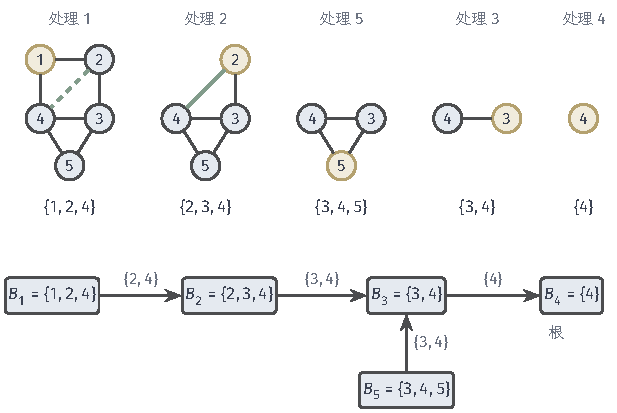
\includegraphics[width=104.369mm]{figures/01-basic-mathematics/04-graphs/tikz/c5-elimination-to-decomposition/figure.pdf}
  \caption{由消元次序$(1,2,5,3,4)$构造树分解。上行：每一轮的当前图，黄色为正在处理的顶点，绿色虚线为本轮补入的填充边，下一轮中它以绿色实线留在当前图里；图下标出记录的袋。下：按“连到最早被处理的后续邻居”连接父袋得到的袋树，箭头指向父袋，边旁标出接口。}
  \label{fig:graph-dp-elimination-to-decomposition}
\end{figure}

表中每个非根袋与父袋的接口恰好等于它的后续邻居集合。这不是巧合：父袋容纳$S_v$，而$v$本身比父袋的顶点都早被处理，不在父袋中，所以$B_v\cap B_{p(v)}=S_v$。第~\ref{sec:graph-dp-function-message-correspondence}小节会利用这一点把中间函数与袋之间的消息对应起来。

\subsection{从消元簇得到树分解}
\label{sec:graph-dp-clusters-to-decomposition}

下面的定理说明上述构造总是给出树分解，从而把消元过程中生成的依赖正式转成树分解，而不是另设一套独立的构建方法。

\begin{theorem}[消元次序产生树分解]
\label{thm:graph-dp-elimination-decomposition}
设$\mathcal G$是非空有限无向图，$R\subseteq V$，$\pi$是$V\setminus R$的消元次序。按算法~\ref{alg:graph-dp-order-to-decomposition}得到的袋树是$\mathcal G_R$的树分解，有保留集时根袋$B_R=R$；其宽度为$\pi$的诱导宽度与$|R|-1$中的较大者，无保留集时就是诱导宽度。特别地，$\mathcal G$的树宽不超过任何完整消元次序的诱导宽度。
\end{theorem}

\begin{proof}
先说明袋树是树。每个非根袋恰有一条通向父袋的边。父袋若为$B_{p(v)}$，则$p(v)$在次序中排在$v$之后，沿父边前进时次序位置严格增大；父袋若为$B_R$，则到达根袋。所以沿父边前进不会回到出发点，不形成环，每条父链都在有限步后到达一个根。各根之间再用树边连接，整体连通且无环。

顶点覆盖：待消去的$v$属于$B_v$，$R$中的顶点属于$B_R$。边覆盖：设$\{u,v\}$是$\mathcal G_R$的边。若两端都在$R$中，它被$B_R$覆盖。否则设$u$是两端中先被处理的待消去顶点；在处理$u$之前，图中只删去过已处理的顶点及其关联边，所以边$\{u,v\}$仍在，$v\in N^+_\pi(u)$，于是$B_u$同时含$u,v$。

运行交集：设$z\in B_v$且$z\neq v$，只需证明从$B_v$沿父链向上的每个袋都含$z$，直到到达$B_z$（$z$待消去时）或$B_R$（$z\in R$时）。这样含$z$的每个袋都与$B_z$或$B_R$由一条全部含$z$的路径相连，$T_z$连通。由$z\in N^+_\pi(v)=S_v$和上一小节的“父袋容纳剩余作用域”，父袋包含$S_v$，所以含$z$；若父袋是$B_{p(v)}$且$p(v)\neq z$，就对$p(v)$重复同样的论证。次序位置严格增大，最终到达$B_z$或$B_R$。

宽度：待消去顶点的袋大小为$|S_v|+1$，根袋大小为$|R|$，所以宽度如定理所述。最后，无保留集时树宽是全部树分解宽度的最小值，所以不超过诱导宽度。
\end{proof}

证明中的边覆盖论证同样适用于填充边，因此所得袋树也是填充图$\mathcal G^+_\pi$的树分解。

另一个直接推论是：每个局部函数的作用域$S_a$都整体落在某个袋中。取$S_a$中最先被处理的待消去变量$v$，$S_a$的其余变量在原始图中都与$v$相邻且排在$v$之后（或属于$R$），所以都在$S_v$中，$S_a\subseteq B_v$；若$S_a\subseteq R$，则$S_a\subseteq B_R$。第~\ref{sec:graph-dp-term-assignment}小节据此为局部项指定归属。

\paragraph{结构操作的代价}
设处理第$t$个顶点时它有$d_t$个当前邻居，补边要检查$\sum_t d_t(d_t-1)/2$对顶点，记录的袋共含$\sum_t(d_t+1)$个顶点。用支持常数时间查边和加边的邻接集合实现时，时间为
\[
O\Bigl(n+m+\sum_t d_t^2\Bigr),
\]
其中$m$是原始图的边数。这只是结构操作的开销；在袋上计算数值表时，开销随袋大小指数增长，第~\ref{sec:graph-dp-computation-cost}节另行计算。
